\documentclass[
  bibliography=totoc,     % Literatur im Inhaltsverzeichnis
  captions=tableheading,  % Tabellenüberschriften
  titlepage=firstiscover, % Titelseite ist Deckblatt
]{scrartcl}


% Paket float verbessern
\usepackage{scrhack}

% Warnung, falls nochmal kompiliert werden muss
\usepackage[aux]{rerunfilecheck}

% unverzichtbare Mathe-Befehle
\usepackage{amsmath}
% viele Mathe-Symbole
\usepackage{amssymb}
% Erweiterungen für amsmath
\usepackage{mathtools}

% Fonteinstellungen
\usepackage{fontspec}
% Latin Modern Fonts werden automatisch geladen
% Alternativ:
%\setromanfont{Libertinus Serif}
%\setsansfont{Libertinus Sans}
%\setmonofont{Libertinus Mono}
\recalctypearea % Wenn man andere Schriftarten gesetzt hat,
% sollte man das Seiten-Layout neu berechnen lassen

% deutsche Spracheinstellungen
\usepackage{polyglossia}
\setmainlanguage{german}


\usepackage[
  math-style=ISO,    % ┐
  bold-style=ISO,    % │
  sans-style=italic, % │ ISO-Standard folgen
  nabla=upright,     % │
  partial=upright,   % ┘
  warnings-off={           % ┐
    mathtools-colon,       % │ unnötige Warnungen ausschalten
    mathtools-overbracket, % │
  },                       % ┘
]{unicode-math}

% traditionelle Fonts für Mathematik
\setmathfont{Latin Modern Math}
% Alternativ:
%\setmathfont{Libertinus Math}

\setmathfont{XITS Math}[range={scr, bfscr}]
\setmathfont{XITS Math}[range={cal, bfcal}, StylisticSet=1]

% Zahlen und Einheiten
\usepackage[
  locale=DE,                   % deutsche Einstellungen
  separate-uncertainty=true,   % immer Fehler mit \pm
  per-mode=symbol-or-fraction, % / in inline math, fraction in display math
]{siunitx}

% chemische Formeln
\usepackage[
  version=4,
  math-greek=default, % ┐ mit unicode-math zusammenarbeiten
  text-greek=default, % ┘
]{mhchem}

% richtige Anführungszeichen
\usepackage[autostyle]{csquotes}

% schöne Brüche im Text
\usepackage{xfrac}

% Standardplatzierung für Floats einstellen
\usepackage{float}
\floatplacement{figure}{H}
\floatplacement{table}{H}

% Floats innerhalb einer Section halten
\usepackage[
  section, % Floats innerhalb der Section halten
  below,   % unterhalb der Section aber auf der selben Seite ist ok
]{placeins}

%dassselbe für Subsections 
\makeatletter
\AtBeginDocument{%
  \expandafter\renewcommand\expandafter\subsection\expandafter{%
    \expandafter\@fb@secFB\subsection
  }%
}
\makeatother

% Seite drehen für breite Tabellen: landscape Umgebung
\usepackage{pdflscape}

% Captions schöner machen.
\usepackage[
  labelfont=bf,        % Tabelle x: Abbildung y: ist jetzt fett
  font=small,          % Schrift etwas kleiner als Dokument
  width=0.9\textwidth, % maximale Breite einer Caption schmaler
]{caption}
% subfigure, subtable, subref
\usepackage{subcaption}

% Grafiken können eingebunden werden
\usepackage{graphicx}
% größere Variation von Dateinamen möglich
\usepackage{grffile}

% schöne Tabellen
\usepackage{booktabs}

% Verbesserungen am Schriftbild
\usepackage{microtype}

% Literaturverzeichnis
\usepackage[
  backend=biber,
]{biblatex}
% Quellendatenbank
\addbibresource{programme.bib}

% Hyperlinks im Dokument
\usepackage[
  unicode,        % Unicode in PDF-Attributen erlauben
  pdfusetitle,    % Titel, Autoren und Datum als PDF-Attribute
  pdfcreator={},  % ┐ PDF-Attribute säubern
  pdfproducer={}, % ┘
]{hyperref}
% erweiterte Bookmarks im PDF
\usepackage{bookmark}

% Trennung von Wörtern mit Strichen
\usepackage[shortcuts]{extdash}

%selbst hinzugefügt
\usepackage{physics}

\title{V703 - Das Geiger-Müller-Zählrohr}
\date{Durchführung: 28.05.2019, Abgabe: 04.06.2019}
\author{
  Jan Herdieckerhoff
  \texorpdfstring{%
    \\%
    \href{mailto:jan.herdieckerhoff@tu-dortmund.de}{jan.herdieckerhoff@tu-dortmund.de}
  }{}%
  \texorpdfstring{\and}{, }
  Karina Overhoff
  \texorpdfstring{%
    \\%
    \href{mailto:karina.overhoff@tu-dortmund.de}{karina.overhoff@tu-dortmund.de}
  }{}%
}
\publishers{TU Dortmund – Fakultät Physik}

\begin{document}
\maketitle
\tableofcontents
\newpage
\section{Ziel}
Ziel dieses Versuches ist es, die Elastizitätsmodule
verschiedener Stäbe durch Messung ihrer Biegung
zu bestimmen.
\section{Theorie}
%Spannung
Die Spannung ist die Kraft auf einen Körper pro Flächeneinheit.
Die Komponente, die senkrecht zur Oberfläche steht,
ist die Normalspannung $\sigma$. Ihre oberflächenparallele
Komponente heißt Tangentialspannung.
%Hookesches Gesetz
Das Hookesche Gesetz stellt den Zusammenhang zwischen
der Spannung $\sigma$, die am Körper angreift, und der
Deformation des Körpers dar:
\begin{equation}
\sigma = E \frac{\Delta L}{L}
\label{eqn:Hooke}
\end{equation}
%Elastizitätsmodul
$E$ ist dabei das Elastizitätsmodul.
Das Elastizitätsmodul ist eine Materialkonstante, die
anhand der Deformation eines Körpers bestimmt werden kann.
%Biegung
Eine Art der Deformation ist die Biegung. Sie entsteht, wenn
eine Kraft, wie in Abbildung 1 und in Abbildung 2 gezeigt, auf einen Körper wirkt. %Abbildung 1 erwähnen
%Berechnung der Durchbiegung, einseitig
Zunächst wird die Berechnung der Biegung eines Stabes bei einseitiger
Einspannung beschrieben. %Abbildung 1
\begin{figure}
    \centering
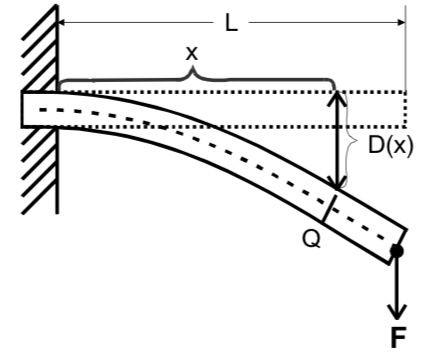
\includegraphics[width= 10cm, height= 5cm]{./plots/abb1.png}
\caption{}
\label{fig:abb1}
\end{figure}
Die Durchbiegung $D(x)$ bezeichnet die Verschiebung eines Oberflächenpunktes
an der Stelle x zwischen dem belasteten und unbelasteten Zustand des Stabes.
Es wird eine Drehmomentgleichung aufgestellt, um $D(x)$ zu bestimmen.
Die Zug- und Druckspannungen, die an der Querschnittsfläche $Q$ angreifen,
sind entgegesetzt gleich und bewirken deshalb ein Drehmoment $M_{\sigma}$:
\begin{equation*}
M_{\sigma} = \int_{Q} y \sigma(y) dq
\end{equation*}
$y$ ist der Abstand des Flächenelementes $dq$ von der neutralen
Faser. Die neutrale Faser ist die Fläche, in der keine Spannungen
auftreten. Ihre Länge ändert sich bei der Biegung folglich nicht.
Ein weiteres Drehmoment $M_{F}$ entsteht durch die Kraft auf einen senkrecht
zur Stabachse stehenden Querschnitt. Es verdreht den Querschnitt aus 
seiner ursprünglichen vertikalen Lage.
Die Deformation des Körpers stellt sich so ein, dass die Drehmomente an
jeder Stelle $x$ übereinstimmen:
\begin{equation*}
M_{F} = M_{\sigma}.
\end{equation*}
Dabei ist
\begin{equation*}
M_{F} = F (L-x),
\end{equation*}
da die Kraft $F$ über den Hebelarm $L-x$ an $Q$ angreift.
Damit ist das Gleichgewicht der Drehmomente durch
\begin{equation}
\int_{Q} y \sigma(y) dq = F(L-x)
\label{eqn:Momente}
\end{equation}
gegeben.
Mit dem Hookeschen Gesetz \eqref{eqn:Hooke} wird die Normalspannung
$\sigma(y)$ mittels
\begin{equation*}
\sigma(y) = E \frac{\delta x}{\Delta x}
\end{equation*}
berechnet. Hier ist $\Delta x$ die Länge eines kurzen Stabstücks
und $\delta x$ die Längenänderung der Faser.
Es gilt außerdem
\begin{equation*}
\delta x = y \Delta \phi = y \frac{\Delta x}{R},
\end{equation*}
wobei $R$ der Krümmungsradius der Faser bei $x$ ist.
Damit ist
\begin{equation*}
\sigma(y) = E \frac{y}{R} = E y \frac{d^2D}{dx^2},
\end{equation*}
da für geringe Kurvenkrümmungen
\begin{equation*}
\frac{1}{R} \approx \frac{d^2D}{dx^2}
\end{equation*}
gilt, falls
\begin{equation*}
(\frac{dD}{dx})^2 << 1
\end{equation*}
ist. Für \eqref{eqn:Momente} ergibt sich damit:
\begin{equation}
E \frac{d^2D}{dx^2} \int_{Q} y^2 dq = F(L-x).
\label{eqn:Momente2}
\end{equation}
Dabei ist
\begin{equation*}
I = \int_{Q} y^2 dq(y)
\end{equation*}
das Flächenträgheitsmoment.
Integriert man \eqref{eqn:Momente2} und stellt die Gleichung
nach $D(x)$ um, erhält man für die Biegung bei einseitiger Einspannung
\begin{equation}
D(x) = \frac{F}{2EI} (Lx^2- \frac{x^3}{3}).
\label{eqn:D1}
\end{equation}
Diese Gleichung ist für $0 \leq x \leq L$ definiert.
Die Integrationskonstanten verschwinden, weil $D(0) = 0$ und $\frac{dD}{dx} = 0$ sein müssen.

\begin{figure}
    \centering
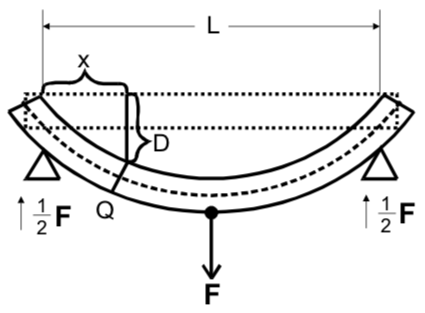
\includegraphics[width= 10cm, height= 5cm]{./plots/abb2.png}
\caption{}
\label{fig:abb2}
\end{figure}
%Berechnung der Durchbiegung, zweiseitig
\noindent Liegen beide Stabenden auf und lässt man in der Mitte des Stabes
eine Kraft angreifen, greift an der Querschnittsfläche die Kraft
$\frac{F}{2}$ mit dem Hebelarm $x$ an. Für die erste Stabhälfte $0 \leq x \leq \frac{L}{2}$
gilt für das Drehmoment
\begin{equation*}
M_{F} = - \frac{F}{2} x.
\end{equation*}
Für die zweite Hälfte $\frac{L}{2} \leq x \leq L$ gilt
\begin{equation*}
M_{F} = - \frac{F}{2} (L-x).
\end{equation*}
Damit ergibt sich hier für \eqref{eqn:Momente2}
\begin{equation}
\frac{d^2D}{dx^2} = - \frac{F}{EI} \frac{x}{2} \qq{für $0 \leq x \leq \frac{L}{2}$}
\label{eqn:links}
\end{equation}
und
\begin{equation}
\frac{d^2D}{dx^2} = -\frac{1}{2} \frac{F}{EI} (L-x) \qq{für $\frac{L}{2} \leq x \leq L$}.
\label{eqn:rechts}
\end{equation}
Integriert man beide Gleichungen, ergibt sich 
\begin{equation*}
\frac{dD}{dx} = - \frac{F}{EI} \frac{x^2}{4} + C \qq{für $0 \leq x \leq \frac{L}{2}$}
\end{equation*}
und
\begin{equation*}
\frac{dD}{dx} = - \frac{1}{2} \frac{F}{EI} (Lx-\frac{x^2}{2}) + C' \qq{für $\frac{L}{2} \leq x \leq L$}.
\end{equation*}
Da die Biegekurve in der Mitte des Stabes eine horizontale Tangente
haben muss, muss für die Konstanten gelten:
\begin{equation*}
C = \frac{F}{EI} \frac{L^2}{16}
\end{equation*}
und
\begin{equation*}
C' = \frac{3}{16} \frac{F}{EI} L^2.
\end{equation*}
Setzt man die Konstanten in \eqref{eqn:links} und \eqref{eqn:rechts}
ein und integriert die Ausdrücke, erhält man die Gleichungen
für die Biegung bei zweiseitiger Auflage des Stabes:
\begin{equation}
D(x) = \frac{F}{48EI} (3L^2x - 4x^3) \qq{für $0 \leq x \leq \frac{L}{2}$}
\label{eqn:D2links}
\end{equation}
und
\begin{equation}
D(x) = \frac{F}{48EI} (4x^3 - 12Lx^2 + 9L^2x - L^3) \qq{für $\frac{L}{2} \leq x \leq L$}.
\label{eqn:D2rechts}
\end{equation}
Die Integrationskonstanten verschwinden hier, weil $D(0) = 0$ und $D(L) = 0$ sein müssen.
Die Biegung eines elastischen Stabes kann also durch
\eqref{eqn:D1}, \eqref{eqn:D2links} und \eqref{eqn:D2rechts} bestimmt werden.

%D(x)=D_M(x)-D_0(x)
\noindent Weil die Stäbe nicht als exakt gerade angenommen werden können,
muss die Biegung ohne angehängtes Gewicht gemessen werden.
Die Biegung des Stabes durch die Last ist dann 
\begin{equation}
D(x) = D_{M}(x) - D_{0}(x).
\label{eqn:D(x)}
\end{equation}

%Lineare Regression, Berechnung von E
\noindent Der Elastizitätsmodul lässt sich mittels einer
linearen Regression bestimmen. Die Werte für die Biegung \eqref{eqn:D(x)}
werden gegen eine liearisierte Form des horizontalen Abstands aufgetragen.
Diese können aus den Gleichungen \eqref{eqn:D1}, \eqref{eqn:D2links} und \eqref{eqn:D2rechts} entnommen werden.
Die Steigung berechnet sich dabei wie folgt:
\begin{equation}
m = \frac{\overline{xy} - \overline{x} \cdot \overline{y}}{\overline{x^2} - \overline{x}^2}.
\label{eqn:m}
\end{equation} %MW etc auch erwähnen?
Bei dem ersten und zweiten Stab entspricht die Steigung
$\frac{F}{2EI}$.
Stellt man den Ausdruck nach $E$ um, erhält man
eine Gleichung für den Elastizitätsmodul:
\begin{equation}
E = \frac{F}{2mI}.
\label{eqn:E12}
\end{equation}
Für den dritten Stab ergibt sich für den Elastizitätsmodul auf die
selbe Weise die Gleichung:
\begin{equation}
E = \frac{F}{48mI}.
\label{eqn:E3}
\end{equation}

\section{Durchführung}
Die Apparatur ist in Abbildung xy zu sehen. %Abbildung Apparatur erwähnen
Die Stäbe werden entweder einseitig eingeklemmt oder zweiseitig
auf den Punkten $A$ und $B$ gelagert. Die Stäbe werden belastet, indem
ein Gewicht entweder am Stabende oder in der Stabmitte angehängt wird.
Die Biegung wird mit zwei Messuhren, die sich auf einer Längen-Skala befinden
und verschiebbar sind, sodass die Biegung an verschiedenen Stellen $x$ bestimmt
werden kann, gemessen. Bei Messuhren wird die Verschiebung eines Objektes mittels
eines federnden Taststiftes gemessen. %andere Formulierung
%Hier Abbildung einfügen
\begin{figure}
    \centering
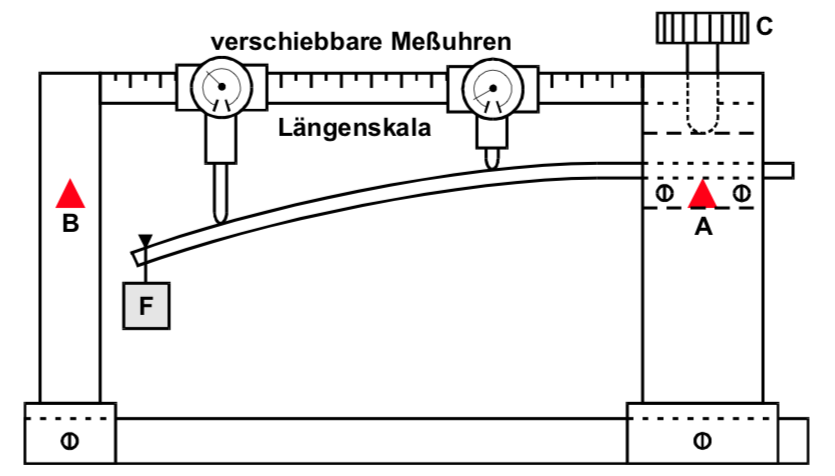
\includegraphics[width= 10cm, height= 5cm]{./plots/abb3.png}
\caption{}
\label{fig:abb3}
\end{figure}

Zunächst wird jeweils für zwei einseitig eingespannte Stäbe die Biegung ohne
angehängtes Gewicht gemessen. Danach wird an das Stabende ein Gewicht angehängt.
Die Biegung wird mit einer der Messuhren gemessen. %Abbildung einseitiger Stab
Ein dritter Stab wird
zweiseitig aufgelegt. Es wird wieder zunächst die Biegung ohne Gewicht und dann
mit Gewicht gemessen. Hier wird für die erste Hälfte des Stabes $\frac{L}{2} \leq x \leq L$
die linke Messuhr und für die zweite Hälfte $0 \leq x \leq \frac{L}{2}$ die rechte Messuhr
verwendet. %Abbildung zweiseitiger Stab
Zuletzt werden die Längen, Breiten, beziehungsweise Durchmesser und Massen der Stäbe,
sowie die Masse des angehängten Gewichts bestimmt.

\newpage
\section{Auswertung}
\label{sec:Auswertung}

\subsection{Bestimmung des Elastizitätsmoduls des ersten Stabes}
% Tabellen und Plot zu E1, erste Stange
\begin{table}\caption{Gewicht, Länge und Durchmesser des ersten Stabs}
\label{table: Stab1}
\centering
\sisetup{round-mode = places, round-precision=2, round-integer-to-decimal=true}
\begin{tabular}{S[]S[]S[]} 
\toprule
{Gewicht$/\si{\gram}$} & {Länge$/\si{\centi\meter}$} & {Durchmesser$/\si{\milli\meter}$}\\
\midrule
460.3 & 51.2 & 8.0\\
\bottomrule
\end{tabular}\end{table}

Die Biegung $D(x)$ an den Stellen $x$ mit und ohne Gewicht
ist für den ersten Stab in \ref{table: D1} zu sehen. Die Biegung ist
jeweils in $\si{\mm}$ angegeben.
Die horizontale Länge $x$ ist in $\si{\cm}$ angegeben.
\begin{table}\caption{}
\label{}
\centering
\sisetup{round-mode = places, round-precision=2, round-integer-to-decimal=true}
\begin{tabular}{S[]S[]S[]} 
\toprule
{$D(x)/\si{\milli\meter}$ ohne Gewicht} & {$D(x)/\si{\milli\meter}$ mit Gewicht} & {$x/\si{\centi\meter}$}\\
\midrule
0.98 & 1.1 & 3.0\\
1.04 & 1.1 & 5.0\\
1.11 & 1.17 & 8.0\\
1.16 & 1.17 & 11.0\\
1.12 & 1.18 & 14.0\\
1.12 & 1.19 & 17.0\\
1.1 & 1.19 & 20.0\\
1.03 & 1.21 & 23.0\\
0.93 & 1.23 & 26.0\\
0.8 & 1.24 & 29.0\\
0.68 & 1.25 & 32.0\\
0.58 & 1.25 & 35.0\\
0.4 & 1.25 & 38.0\\
0.2 & 1.26 & 41.0\\
0.08 & 1.26 & 44.0\\
-0.1 & 1.26 & 47.0\\
-0.38 & 1.26 & 49.0\\
\bottomrule
\end{tabular}\end{table}
Die Differenz \eqref{eqn:D(x)} der beiden Biegungen aus \ref{table: D1} 
und die jeweiligen horizontalen Abstände in linearisierter Form $Lx^2-\frac{x^3}{3}$
sind in \ref{table: new1} dargestellt.
\begin{table}\caption{}
\label{}
\centering
\sisetup{round-mode = places, round-precision=2, round-integer-to-decimal=true}
\begin{tabular}{S[]S[]} 
\toprule
{$D(x)/m$ Differenz} & {$Lx^2-x^3/3 /m^3$}\\
\midrule
0.00012000000000000011 & 0.0004751999999999999\\
6.0000000000000056e-05 & 0.0013033333333333334\\
5.999999999999983e-05 & 0.003272533333333333\\
1.000000000000001e-05 & 0.006066133333333332\\
5.999999999999983e-05 & 0.009630133333333332\\
6.999999999999984e-05 & 0.013910533333333334\\
8.999999999999986e-05 & 0.018853333333333333\\
0.00017999999999999993 & 0.024404533333333332\\
0.0002999999999999999 & 0.03051013333333333\\
0.00043999999999999996 & 0.03711613333333332\\
0.00057 & 0.04416853333333332\\
0.00067 & 0.05161333333333332\\
0.00085 & 0.05939653333333332\\
0.00106 & 0.06746413333333331\\
0.0011799999999999998 & 0.07576213333333331\\
0.00136 & 0.08423653333333331\\
0.0016400000000000002 & 0.08995746666666665\\
\bottomrule
\end{tabular}\end{table}

Auf diese Weise lässt sich mit Hilfe des Graphen %Plot1
der Elastizitätsmodul durch die Steigung bestimmen.
\begin{figure}
  \centering
  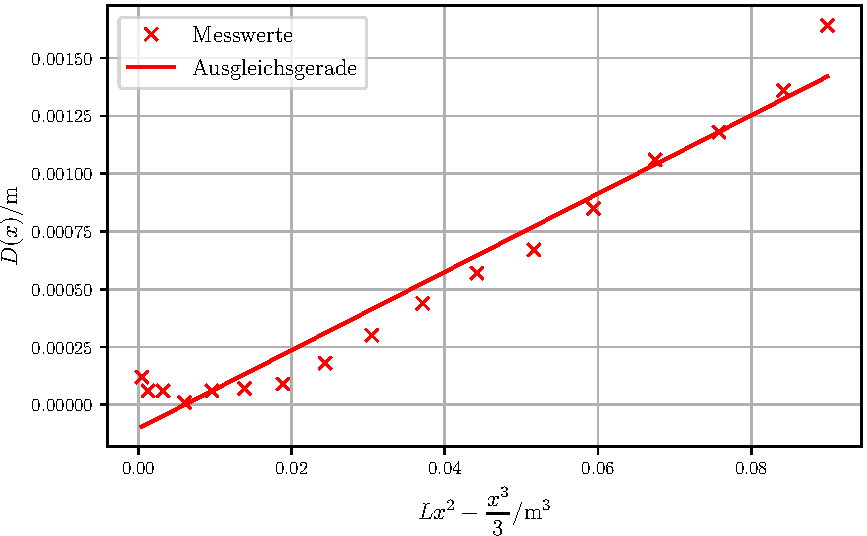
\includegraphics[width=12cm, height=9cm]{./plots/Stange1.pdf}
  \caption{Auftragung der Differenzen der vertikalen Abstände des Stabes mit und ohne Gewicht gegen die horizontalen Abstände in linearisierter Form mit zusätzlicher Ausgleichsgeraden}
  \label{fig:plot1}
\end{figure}
Die Steigung ergibt sich mit \eqref{eqn:m}
zu $m = \SI{0.016939}{\meter}$. Damit ist der Elastizitätsmodul mit \eqref{eqn:E12}%1/m²
$E = \SI{459.04}{\giga\pascal}$.
\newpage

\subsection{Bestimmung des Elastizitätsmoduls des zweiten Stabes}

\begin{table}\caption{}
\label{}
\centering
\sisetup{round-mode = places, round-precision=2, round-integer-to-decimal=true}
\begin{tabular}{S[]S[]S[]} 
\toprule
{Gewicht$/\si{\gram}$} & {Länge$/\si{\centi\meter}$} & {Durchmesser$/\si{\milli\meter}$}\\
\midrule
121.3 & 53.8 & 8.2\\
\bottomrule
\end{tabular}\end{table}

% Tabellen und Plot zu E2, zweite Stange
In \ref{table: D2} befinden sich die Werte der Biegung $D(x)$
mit und ohne angehängtes Gewicht und die horizontale Auslenkung %Auslenkung?
für den zweiten Stab.
\begin{table}\caption{}Vertikaler Abstand der Stange zur Messuhr mit und ohne Gewicht,
Abstand der Messuhr vom Ursprung auf der horizontalen Achse
\label{table: D2}
\centering
\sisetup{round-mode = places, round-precision=2, round-integer-to-decimal=true}
\begin{tabular}{S[]S[]S[]} 
\toprule
{$D(x)/\si{\milli\meter}$ ohne Gewicht} & {$D(x)/\si{\milli\meter}$ mit Gewicht} & {$x/\si{\centi\meter}$}\\
\midrule
0.87 & 0.79 & 3.0\\
0.91 & 0.77 & 5.0\\
0.98 & 0.68 & 8.0\\
1.01 & 0.5 & 11.0\\
1.03 & 0.27 & 14.0\\
1.03 & -0.05 & 17.0\\
1.04 & -0.42 & 20.0\\
0.96 & -1.3 & 26.0\\
0.88 & -1.83 & 29.0\\
0.82 & -2.42 & 32.0\\
0.69 & -3.13 & 35.0\\
0.55 & -3.71 & 38.0\\
0.36 & -4.41 & 41.0\\
0.1 & -5.23 & 44.0\\
-0.15 & -6.16 & 47.0\\
-0.33 & -6.56 & 49.0\\
\bottomrule
\end{tabular}\end{table}

Die Differenz \eqref{eqn:D(x)} der Biegungen ohne und mit Gewicht und die Abstände in
lineartisierter Form sind in \ref{table: new2} zu sehen.
\begin{table}\caption{}
\label{}
\centering
\sisetup{round-mode = places, round-precision=2, round-integer-to-decimal=true}
\begin{tabular}{S[]S[]} 
\toprule
{D(x) in m} & {x in m³}\\
\midrule
7.999999999999997e-05 & 0.0004518\\
0.00014000000000000001 & 0.0012383333333333337\\
0.0002999999999999999 & 0.0031061333333333337\\
0.00051 & 0.005751533333333333\\
0.00076 & 0.009120533333333333\\
0.00108 & 0.013159133333333335\\
0.00146 & 0.017813333333333337\\
0.00226 & 0.028752533333333333\\
0.00271 & 0.03492953333333333\\
0.00324 & 0.041506133333333334\\
0.00382 & 0.04842833333333334\\
0.00426 & 0.05564213333333334\\
0.004770000000000001 & 0.06309353333333333\\
0.00533 & 0.07072853333333333\\
0.00601 & 0.07849313333333334\\
0.006229999999999999 & 0.08371486666666667\\
\bottomrule
\end{tabular}\end{table}
\begin{figure}

  \centering
  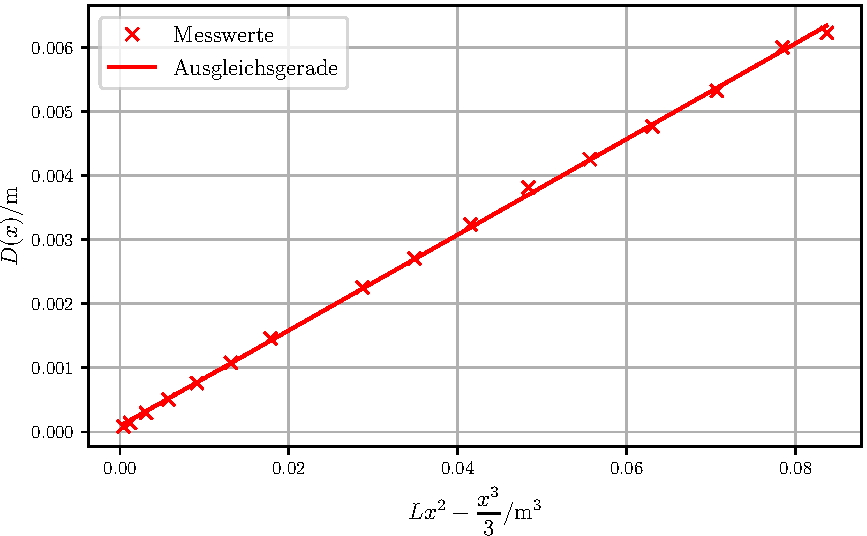
\includegraphics[width=12cm, height=9cm]{./plots/Stange2.pdf}
  \caption{Auftragung der Differenzen der vertikalen Abstände des Stabes m      it und ohne Gewicht gegen die horizontalen Abstände in linearisierter Form       mit zusätzlicher Ausgleichsgeraden}
  \label{fig:plot2}
\end{figure}
Aus der Steigung $m = \SI{0.074685}{\meter}$, die mittels \eqref{eqn:m}
berechnet wurde, ergibt sich der Elastizitätsmodul der zweiten Stange \eqref{eqn:E12} zu
$E = \SI{160.12}{\giga\pascal}$.
\newpage

\subsection{Bestimmung des Elastizitätsmoduls des dritten Stabes}
%Tabellen und Plot zu E3a, dritte Stange
\begin{table}\caption{Gewicht, Länge und Durchmesser des dritten Stabs}
\label{table: Stab3}
\centering
\sisetup{round-mode = places, round-precision=2, round-integer-to-decimal=true}
\begin{tabular}{S[]S[]S[]} 
\toprule
{Gewicht$/\si{\gram}$} & {Länge$/\si{\centi\meter}$} & {Durchmesser$/\si{\milli\meter}$}\\
\midrule
394.3 & 56.1 & 8.0\\
\bottomrule
\end{tabular}\end{table}

Die Werte der rechten Hälfte des dritten Stabes sind in \ref{table: D3a} zu finden.
\begin{table}\caption{}
\label{}
\centering
\sisetup{round-mode = places, round-precision=2, round-integer-to-decimal=true}
\begin{tabular}{S[]S[]S[]} 
\toprule
{D(x)ohne} & {D(x)mit} & {x}\\
\midrule
0.75 & 0.71 & 3.0\\
0.79 & 0.72 & 5.0\\
0.82 & 0.72 & 8.0\\
0.83 & 0.7 & 11.0\\
0.8 & 0.6 & 14.0\\
0.74 & 0.49 & 17.0\\
0.66 & 0.34 & 20.0\\
0.55 & 0.19 & 23.0\\
0.66 & 0.34 & 20.0\\
0.55 & 0.19 & 23.0\\
0.45 & 0.05 & 26.0\\
\bottomrule
\end{tabular}\end{table}
Die Differenz \eqref{eqn:D(x)} der Biegungen ohne und mit Gewicht in der Stabmitte
und die Abstände in linearisierter Form $3L^2x-4x^3$ sind in \ref{table: new3a} aufgelistet.
\begin{table}\caption{}
\label{}
\centering
\sisetup{round-mode = places, round-precision=5, round-integer-to-decimal=true}
\begin{tabular}{S[]S[]} 
\toprule
{$D(x)/m$ Differenz} & {$3L^2x-4x^3 /m^3$}\\
\midrule
4.000000000000004e-05 & 0.02821689000000001\\
7.000000000000006e-05 & 0.04670815000000002\\
9.999999999999998e-05 & 0.07348504000000003\\
0.00013000000000000002 & 0.09853393000000003\\
0.00020000000000000006 & 0.12120682000000006\\
0.00025 & 0.14085571000000005\\
0.00032 & 0.15683260000000007\\
0.00036 & 0.16848949000000008\\
0.00032 & 0.15683260000000007\\
0.00036 & 0.16848949000000008\\
0.0004 & 0.17517838000000008\\
\bottomrule
\end{tabular}\end{table}

\begin{figure}

  \centering
  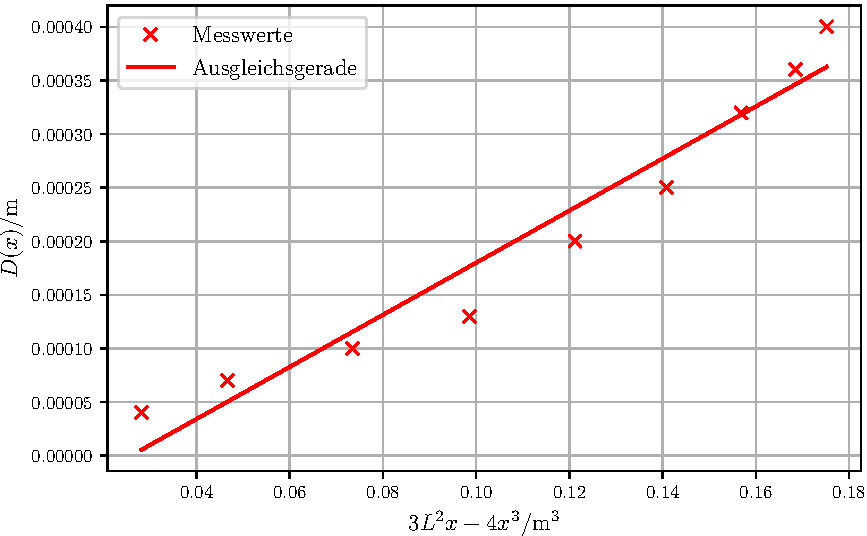
\includegraphics[width=12cm, height=9cm]{./plots/Stange3a.pdf}
  \caption{Auftragung der Differenzen der vertikalen Abstände des Stabes m      it und ohne Gewicht gegen die horizontalen Abstände in linearisierter Form       mit zusätzlicher Ausgleichsgeraden}
  \label{fig:plot3a}
\end{figure}
Mit der Steigung $m = \SI{0.002429}{\meter}$, die mit \eqref{eqn:m}%m 0.002430?
ermittelt wurde, ist der Elastizitätsmodul für die rechte
Hälfte des dritten Stabes \eqref{eqn:E3} $E =\SI{226.35}{\giga\pascal}$.
\newpage

%noch eine subsection?
% Tabellen und Plot zu E3b, dritte Stange
Für die linke Hälfte wurde eine andere Messuhr verwendet.
Die Werte für die Biegungen der linken Hälfte befinden sich in \ref{table: D3b}.
\begin{table}\caption{}
\label{}
\centering
\sisetup{round-mode = places, round-precision=2, round-integer-to-decimal=true}
\begin{tabular}{S[]S[]S[]} 
\toprule
{$D(x)/mm$ ohne Gewicht} & {$D(x)/mm$ mit Gewicht} & {$x/cm$}\\
\midrule
-1.01 & -1.75 & 29.0\\
-0.97 & -1.79 & 32.0\\
-1.08 & -1.89 & 35.0\\
-1.16 & -1.98 & 38.0\\
-1.35 & -2.08 & 41.0\\
-1.48 & -2.13 & 44.0\\
-1.58 & -2.15 & 47.0\\
-1.67 & -2.12 & 50.0\\
-1.76 & -2.06 & 53.0\\
\bottomrule
\end{tabular}\end{table}
Die Differenzen und die linearisierten horizontalen Abstände
$4x^3-12Lx^2+9L^2x-L^3$ finden sich in \ref{table: new3b}.
\begin{table}\caption{}
\label{}
\centering
\sisetup{round-mode = places, round-precision=2, round-integer-to-decimal=true}
\begin{tabular}{S[]S[]} 
\toprule
{$D(x)/\si{\meter}$ Differenz} & {$4x^3-12Lx^2+9L^2x-L^3 /\si{\cubic\meter}$}\\
\midrule
0.00074 & 0.17625812900000004\\
0.0008200000000000001 & 0.1715531990000002\\
0.0008099999999999998 & 0.16164266900000013\\
0.0008200000000000001 & 0.147174539\\
0.00073 & 0.12879680900000012\\
0.0006499999999999999 & 0.10715747900000006\\
0.0005699999999999999 & 0.08290454900000022\\
0.0004500000000000002 & 0.05668601900000003\\
0.00030000000000000003 & 0.029149888999999707\\
\bottomrule
\end{tabular}\end{table}
\begin{figure}

  \centering
  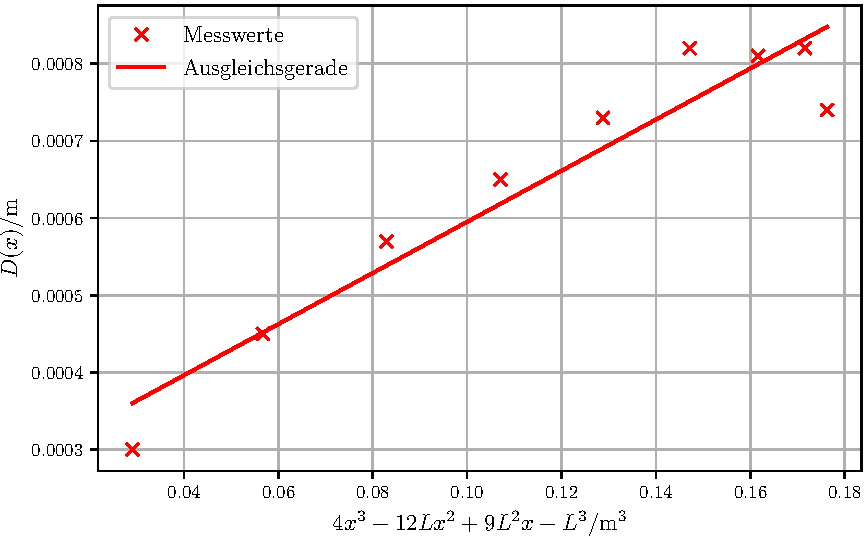
\includegraphics[width=12cm, height=9cm]{./plots/Stange3b.pdf}
  \caption{Auftragung der Differenzen der vertikalen Abstände des Stabes m      it und ohne Gewicht gegen die horizontalen Abstände in linearisierter Form       mit zusätzlicher Ausgleichsgeraden}
  \label{fig:plot3b}
\end{figure}
Der Elastizitätsmodul für die linke Seite des dritten Stabes
errechnet sich mit \eqref{eqn:E3}
mittels der Steigung \eqref{eqn:m}
$m =\SI{0.003312}{\meter}$ zu $E = \SI{166.05}{\giga\pascal}$.

\newpage
\section{Diskussion}
\label{sec:Diskussion}

\subsection{Erster Abstand}

Bei der ersten Messung mit dem Abstand \SI{2.7}{\centi\meter} ergab sich für die Steigung der linearen Ausgleichsrechnung ein relativer Fehler von \SI{0.03}{\percent}. Die mittlere Reichweite hat damit einen relativen Fehler von \SI{0.04}{\percent } und die somit ermittelte Energie hat dann einen relativen Fehler von \SI{0.03}{\percent}. Die durch die Steigung ermittelte Energie hat eine relative Abweichung von \SI{12.57}{\percent}. 

\noindent Für die Steigung der linearen Regression bei dem Plot mit der Energie ergibt sich ein relativer Fehler von \SI{3.67}{\percent}. Somit entspricht dies auch dem relativen Fehler des Energieverlusts der Strahlung. 

\subsection{Zweiter Abstand}

Bei der zweiten Messung mit dem Abstand \SI{2.0}{\centi\meter} ergab sich für die Steigung der linearen Ausgleichsrechnung ein relativer Fehler von \SI{3.67}{\percent}. Die mittlere Reichweite hat damit einen relativen Fehler von \SI{3.65}{\percent } und die somit ermittelte Energie hat also einen relativen Fehler von \SI{2.48}{\percent}. 

\noindent Für die Steigung der linearen Regression bei dem Plot mit der Energie ergibt sich ein relativer Fehler von \SI{2.33}{\percent}. Somit entspricht dies auch dem relativen Fehler des Energieverlusts der Strahlung. Die durch die Steigung ermittelte Energie hat eine relative Abweichung von \SI{30.51}{\percent}. 

\subsection{Vergleich beider Messungen}
Die Reichweiten der ersten und zweiten Messung haben eine relative Abweichung von \SI{65.49}{\percent}. Die sich daraus ergebenden Energien haben eine relative Abweichung von \SI{50.82}{\percent}. Die über die Steigung bestimmten Energien weichen um \SI{38.12}{\percent}.  

\subsection{Statistik des radioaktiven Zerfalls}

Der Fehler des Mittelwerts liegt bei \SI{3.49}{\percent}. 
Die zufällig erzeugten Gauß- und Poisson-Verteilungen sehen der gemessenen Verteilung nicht wirklich ähnlich. Sie sind alle auf eine Höhe normiert. Was aber auffällt, ist, dass in der Mitte der gemessenen Werte eine Lücke vorhanden ist, die genau von der Poisson-Verteilung ausgefüllt wird. Insofern passt die Poisson-Verteilung nicht gut auf das gemessene Ergebnis. Die Gauß-Verteilung passt auch nicht besser, denn sie hat auch nicht die charakteristische Lücke, die unsere Verteilung in der Nähe des Erwartungswertes aufweist. 


%Diskussion: Wert hat sich bei Erschütterung geändert

\nocite{*}
\newpage
\printbibliography
\end{document}
